\section{Results}
\label{sec:results}

The following section discusses the training of the agents and their inference on unseen starting states.
Moreover, the influence of invariant input features on the training success is assessed.
Lastly, the generalization abilities of the trained models to other resolutions and a higher Reynolds number are investigated.%
\footnote{The trained models and the required training files can be obtained from \url{https://github.com/flexi-framework/DRL_LES}.}

\subsection{Training}
\label{sec:results_training}

\begin{figure}[htb!]
  \centering
  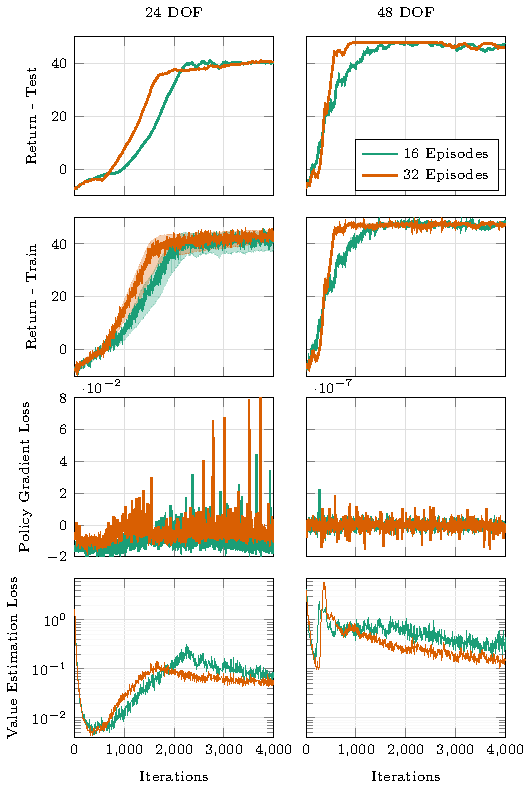
\includegraphics[width=0.99\linewidth]{tikz_double_column/draft-figure2.pdf}
  \caption{Training results for the 24 DOF (left) and 48 DOF (right) test case showing (from top to bottom) the undiscounted collected return on the unseen testing data, the same for the training episodes with the minimum and maximum return indicated by the shaded area, the policy gradient loss according to \eqref{eq:clipping_loss} and the value estimation loss for the value estimation ANN. The results are obtained for either 16 or 32 full episodes used per policy update. Please note that the y-axis of the policy gradient loss is scaled differently for both cases. Since the training simulations update the predictions each $\Delta t_{RL}=0.1$ and are simulated up to $t_{end}=5$, the maximum undiscounted return is $\return_{max}=50$ considering the reward in each step is normalized to $\reward_t\in[-1,1]$.}
  \label{fig:results_training}
\end{figure}


The training took between a single day for the smallest and up to 5 days for the largest cases on the HAWK supercomputer at the High-Performance Computing Center Stuttgart (HLRS).
The training was performed using up to 1024 CPU cores for the simulations and a single GPU node for model execution and training.
For more details on the hardware configuration, the reader is referred to \cite{kurz2022deep}.
The training behavior of the 24 DOF and the 48 DOF configurations is shown exemplarily in \figref{fig:results_training}, since these configurations constitute the lowest and highest employed resolution, respectively.
Both cases were trained once with 16 and with 32 episodes per parameter update.
For all cases, the collected return in the simulation is negative for the randomly initialized policy.
Starting from this initial random policy, the collected return increases during training until the return converges and plateaus just under the maximum undiscounted return of $\return_{max}=50$.
The maximum return follows from the 50 rewards collected during a simulation and the normalization of the reward function in \eqref{eq:reward} that guarantees $r_t\in[-1,1]$.
The convergence of the collected reward indicates that the RL algorithm has found a local optimum with its current policy.
Generally, the gradient estimator used for the gradient ascent algorithm should be more accurate if the amount of sampled episodes per parameter update is increased.
This can speed up the training, since a better approximated gradient can lead to more efficient parameter updates and thus reduce the overall training iterations needed for convergence.
This was indeed observed consistently for all investigated configurations.
Interestingly, the larger 48 DOF case requires less training iterations for convergence compared to the 24 DOF case.
Moreover, the 48 DOF case exhibits less variance in the return sampled in the training runs.
We attribute this reduced variance to two different factors.
First, the influence of the eddy-viscosity model on the overall flow decreases with increasing resolution, since the model accounts for a diminishing amount of unresolved kinetic energy in the flow.
Secondly, a single flow state contains more elements for the larger cases.
Since the policy trains on elementwise data, the same amount of episodes thus provides more training samples for the larger configurations.
The overall reduced variance in the training process then might cause more sample-efficient and faster optimization.
However, since the amount of required iterations for convergence did not decrease consistently with increasing resolution, the faster training might also be simply caused by the stochasticity of the training process.

The last row in \figref{fig:results_training} shows the loss of the value estimation ANN, which is trained to approximate the expected future return starting from a given state of the environment.
The value ANN is initialized with random weights and thus gives a poor estimate of the expected return in the beginning of the training, which results in a high initial loss.
The loss then decreases as the value ANN learns a first sensible estimate of the expected return.
Since the policy then starts to improve, i.e. to collect more reward, also the expected return and thus the training targets of the value ANN change.
Therefore, the value estimation loss increases as the policy improves, since the value ANN has to catch up constantly with the policy.
Once the return reaches a plateau, the expected return as target quantity for the training of the value ANN becomes more stable and the value estimation loss decreases again.


\subsection{Inference}
\label{sec:inference}

\begin{figure*}[htb!]
  \centering
  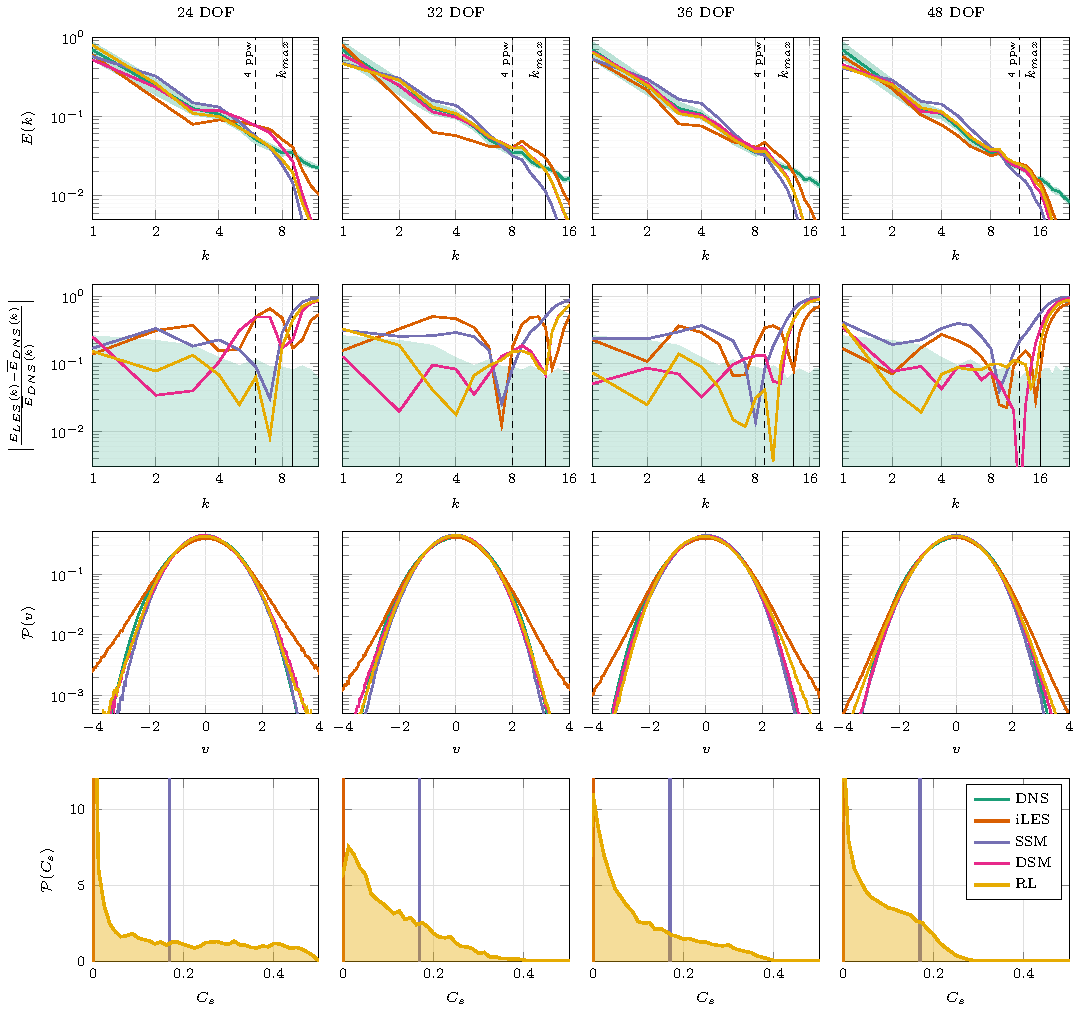
\includegraphics[width=\textwidth]{tikz_double_column/draft-figure3.pdf}
  \caption{Results for the trained RL models (from left to right) in the 24 DOF, 32 DOF, 36 DOF and 48 DOF configuration averaged over $t\in[10,20]$ for an LES initialized with the unseen testing sample. Reported are (from top to bottom) the averaged energy spectra over the wavenumbers $k$, the relative error of the energy spectra with respect to the DNS solution, the distributions $\mathcal{P}(\cdot)$ of the velocity fluctuations, and the distribution of the predicted $C_s$ parameters. The results for the underlying DNS solution as well as an implicitly modeled LES (iLES), the SSM with $C_s=0.17$ and the DSM are shown for comparison. The shaded area for the DNS energy spectrum indicates the maximum and minimum amplitudes observed for each mode. The wavenumber that is resolved by the discretization with 4 points per wavelength is shown dashed and the maximum wavenumber used for optimization $k_{max}$ is indicated with a solid black line.}
  \label{fig:spectra_n5}
\end{figure*}

The performance of the trained RL models is evaluated based on an LES, which is initialized with the unseen testing state and is computed for $t_{end}=20$.
All results reported in the following are obtained and averaged over the timeframe of $t\in[10,20]$.
Since the models are trained only on simulations with $t_{end}=5$, this allows to assess the long-term behavior of the models and whether the simulation time used during training was sufficient.
The results in \figref{fig:spectra_n5} demonstrate that the RL models are indeed long-term stable.
To assess the accuracy of the RL models, they are compared to the SSM and DSM as well as the implicit model.
As could be expected, the implicitly modeled LES exhibits a buildup of energy in the upper wavenumbers due to lacking dissipation.
The SSM with $C_s=0.17$ on the other hand introduces too much dissipation and thus fails to preserve the wavenumbers near the resolution limit of the underlying numerical scheme.
The RL model clearly outperforms both models for all considered configurations by matching the target spectrum almost perfectly up to and even beyond the discretization's resolution limit of around 4 points per wavelength.
The advantage of the RL models is more pronounced for the small cases, where the turbulence model has more impact on the overall flow.
Interestingly, the errors for the different wavenumbers are distributed more evenly for the RL model.
This might stem from the objective of minimizing the squared error in the energy spectrum in order to increase the reward as given in \eqref{eq:reward}. 

The DSM, however, reproduces the DNS spectra with similar accuracy as the RL model.
This is to be expected, since the DSM is known to provide near perfect results for the HIT case, as long as the test filter is situated in the inertial range.
The RL model achieves a similar level of accuracy, i.e. a near optimal policy, without having access to the additional filtering procedure of the DSM.
It is interesting that the most notable difference between the DSM and RL is for the 24 DOF case, where the RL agent provides a significantly better energy spectrum.
A likely explanation for this loss in accuracy of the DSM is that the LES resolution in the 24 DOF case is too coarse for the test filtering to occur in the scale-similar region.
Thus, no meaningful information is provided to the DSM procedure.
The RL model, however, seems to compensate for this lack of resolution and reproduces the DNS spectrum with very good accuracy.
It is important to stress here once again, that the underlying forcing of the test case prescribes the overall energy budget of the simulation.
Therefore, errors in the high wavenumbers might influence the energy contained in the low wavenumber and vice versa.
This stresses the capabilities of the RL models even more, which have learned to interact with this forcing such that the energy spectrum fits the prescribed one based on local information of the flow field only.

\begin{figure*}
  \centering
  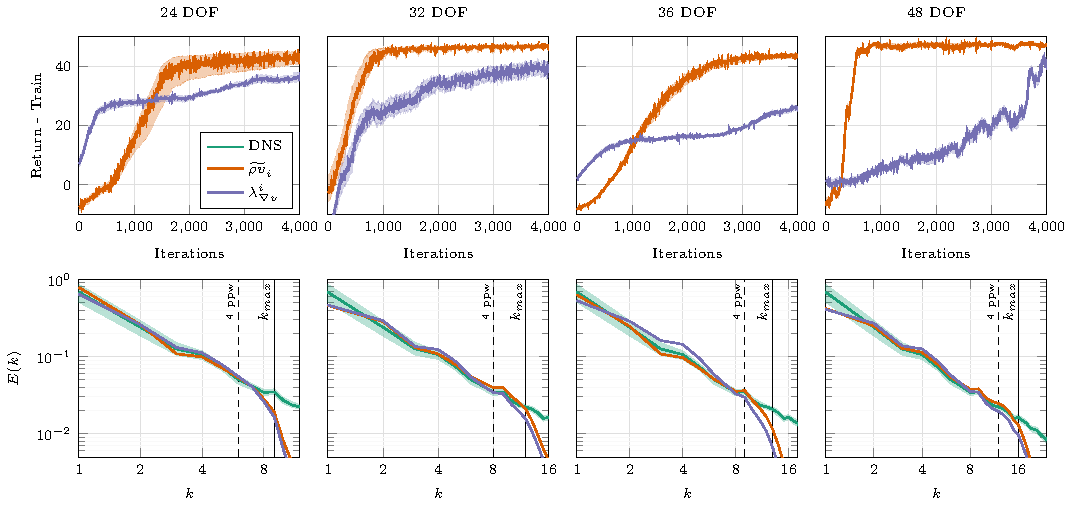
\includegraphics[width=\textwidth]{tikz_double_column/draft-figure4.pdf}
  \caption{Comparison between the RL models trained with the local momentum field $\widetilde{\rho v}_i$ and with the invariants of the velocity gradient tensor $\lambda_{\nabla v}^i$ as inputs for the (from left to right) 24 DOF, 32 DOF, 36 DOF and 48 DOF configuration. The top row shows the undiscounted return collected during training with the shaded area indicating the episodes with the maximum and minimum return. The lower row shows the energy spectra in comparison to the DNS solution. The shaded area in the spectra indicates the maximum and minimum observed energy contained in the respective wavenumber during the DNS. The wavenumber that is resolved by the discretization with 4 points per wavelength is shown dashed and the maximum wavenumber used for optimization $k_{max}$ is indicated with a solid black line.}
  \label{fig:invariants}
\end{figure*}

It seems important to stress again that the energy spectra are the optimization target for the training and thus might provide only limited insight into the model's overall ability to reproduce the required turbulent statistics.
To this end, the distributions of the velocity fluctuations produced by the different models are investigated as additional important measure of the models' performance.
The differences between the models observed here are consistent with the obtained energy spectra.
Since additional dissipation tends to reduce velocity fluctuations, the SSM exhibits the narrowest and the implicit LES the broadest distribution.
For all cases, the velocity fluctuations produced by the RL model appear to be balanced between both effects, since they follow the DNS distribution more closely than the SSM for small fluctuations in the center of the distribution, but do not exhibit the overpronounced tails observed for the implicit LES.
However, the RL model produces an unsymmetrical distribution of velocity fluctuations for the 36DOF case.
This behavior was not observed for any other configuration or model and its origin is still subject of on-going investigations.
It is also unclear whether this behavior emerges since the symmetry condition has to be learned by the model implicitly during the training and might be not strict enough or whether this effect emerges from the long-term interactions between the agent and the forcing method.

The distributions of $C_s$ in the bottom row of \figref{fig:spectra_n5} show qualitatively similar results for all cases.
Most predictions are close to zero with an decreasing amount of higher values.
The overall range seems to strongly depend on the resolution, since the agent exploits almost all of its available action space for the 24 DOF case performing actions near the prescribed maximum of 0.5.
In contrast, the largest $C_s$ prediction for the 48 DOF case does not exceed 0.3.
The predictions' mean thus decreases for increasing resolutions as is consistent with the understanding of an increased LES resolution on the Smagorinsky model.
This difference might stem either from the policy itself, i.e. the policies learned indeed different distributions, or from the input data of the respective resolutions, which might exhibit different distributions.
Nonetheless, these results show the flexibility and capability of the RL training approach to incorporate physical constraints into the model through the choice of the input features.
We did not adapt the expressivity of the ANN between the two input selections, which might increase the performance.

Sarghini et al. \cite{sarghini2003neural} and Maulik et al. \cite{maulik2021deploying} reported a speedup by applying ANN instead of the computationally expensive DSM.
To this end, we compared the computational time required to evaluate the policy and the dynamic procedure of the DSM on a single CPU core for the 48 DOF case.
We found that the time required was comparable for both cases with the RL policy requiring around 10 per cent more time on our hardware.
These results are encouraging, since we did not perform any optimizations of the policy in terms of computational efficiency or model size and did not use GPU acceleration for this comparison, which improves the performance of the RL-based policy significantly.

\subsection{Input Features}
\label{sec:results_features}

In a next step, the models trained on the local momentum field as inputs are compared to the models trained on the five invariants of the velocity gradient tensor $\lambda_{\nabla u}^i$.
The results in \figref{fig:invariants} indicate that again all models successfully improve during training.
However, the training is generally slower and less stable than the former models.
As a result, the final models using the invariants as inputs still partly improve over the analytical models, but perform worse than the models using the momentum field, especially in the 36 DOF case.
This indicates that it is generally harder to learn a sensible policy from the invariants.
To investigate this further, we increased the training time.
While the models always seemed to improve to some degree, even with double the amount of training iterations the gap to former models stayed quite substantial.

We attribute this to the different distributions of the input quantities.
For the considered HIT test case, the velocity fluctuations have zero mean and a root-mean-squared (RMS) magnitude of unity by construction.
The fluctuations are thus approximately normally distributed with zero mean and unit variance.
This is the optimal distribution for input quantities in machine learning, which typically has to be achieved by normalizing the inputs accordingly.
Since the velocity fluctuations are intrinsically linked to the energy budget in the simulation and are thus constraint by the forcing, the agent's actions have only relatively limited impact on the distribution of velocity fluctuations, as already shown in \figref{fig:spectra_n5}.
In contrast, the invariants of the velocity gradient tensor typically span orders of magnitude.
Moreover, the computation of the gradients, and thus the distribution of the invariants, differ widely depending on the employed numerical discretization.
For DG, the gradients are intrinsically discontinuous across element faces and are also known to produce large gradients at the element faces for underresolved turbulence.
This is especially problematic for the initial states, which are obtained by projecting the DNS flow field onto the DG basis with respective LES resolution.
This projection causes large gradients and thus large values for the invariants, which makes it hard to normalize them to a tamer distribution.
We thus assume that the problems in the training stem from the gradient computation of the DG method, for which the gradients exhibit a complex distribution and the invariants computed from it span orders of magnitude, which makes training more difficult for the agent.


\subsection{Generalization to other Resolutions}
\label{sec:results_generalize}

\begin{figure}
  \centering
  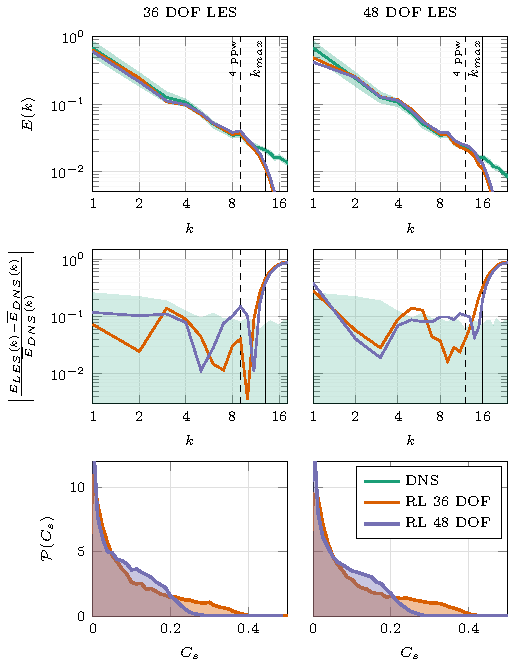
\includegraphics[width=0.99\linewidth]{tikz_double_column/draft-figure5.pdf}
  \caption{Results for the RL model trained on the 48 DOF evaluated on the 36 DOF case (left) and vice versa (right). Given are the energy spectra over the wavenumbers $k$ (top), the error of the spectra in comparison to the DNS solution (center) and the distribution of the predicted $C_s$ parameters (bottom). The shaded area indicates the maximum and minimum observed energy contained in the respective wavenumber during the DNS. The wavenumber that is resolved by the discretization with 4 points per wavelength is shown dashed and the maximum wavenumber used for optimization $k_{max}$ is indicated with a solid black line.}
  \label{fig:generalization_resolution}
\end{figure}

To demonstrate that the trained models can generalize to different resolutions, the model trained on the 48 DOF resolution is evaluated on the 36 DOF configuration and vice versa.
This allows to assess how well the trained models can be transferred to LES cases with either more or less resolution.
The results shown in \figref{fig:generalization_resolution} demonstrate that the trained models can also provide stable and accurate results in LES with different resolutions.
This is especially remarkable, since the policy's field of vision for the policy shrinks with increasing resolution due to the elementwise input and output quantities.
The RL model trained natively on the 48 DOF case shows a slight increase in energy in the higher wavenumbers, while the 36 DOF model seems to be slightly more dissipative.
However, the overall errors in the energy spectrum appear to be comparable for both cases.
The classical turbulence models are not shown for clarity.
However, since both RL models provide almost identical energy spectra, they still outperform the SSM and implicit LES model for both resolutions, while matching the performance of the DSM.

Also, the distribution of the models' predictions are almost identical for both cases and thus do not appear to change depending on the LES resolution.
The predictions of the 36 DOF model exhibit a much wider tail, with a maximum prediction of around $C_{s,max}=0.4$.
In contrast, the predictions of the trained 48 DOF model do not exceed $C_{s,max}=0.3$.
Interestingly, the models are still able to reproduce the target energy spectrum despite the deviations in their policies.
It is plausible to assume that the models will generalize even better, if they are trained on a variety of different resolutions, instead of only a single one.
These pronounced differences in the learned policies indicate that the distribution of predictions is not only induced by the input features but is a characteristic property of the policy trained on the respective resolution and the employed discretization.
This again demonstrates that the different discretizations induce different implicit LES filters, which again require different policies to match the underlying energy spectrum.
Thus, the proposed framework allows to develop discretization-adapted turbulent models for implicit LES.

\subsection{Generalization to other Reynolds Numbers}
\label{sec:results_generalize_re}

In a final step, we demonstrate that the trained RL policy is able to generalize to higher Reynolds numbers.
For this, the trained agents for the different resolutions are applied to a HIT flow at a Reynolds number of $Re_{\lambda}\approx 240$, which is considerably higher than the Reynolds number $Re_{\lambda}\approx 180$ used for training.
Analogously to \secref{sec:inference}, the LES were initialized from filtering the DNS flow field at a random point in time to the required resolution.
The LES was then advanced in time for $t_{end}=20$ and the results were averaged over the timeframe of $t\in [10,20]$ to investigate the long term effects of the model onto the flow.

\begin{figure*}[htb!]
  \centering
  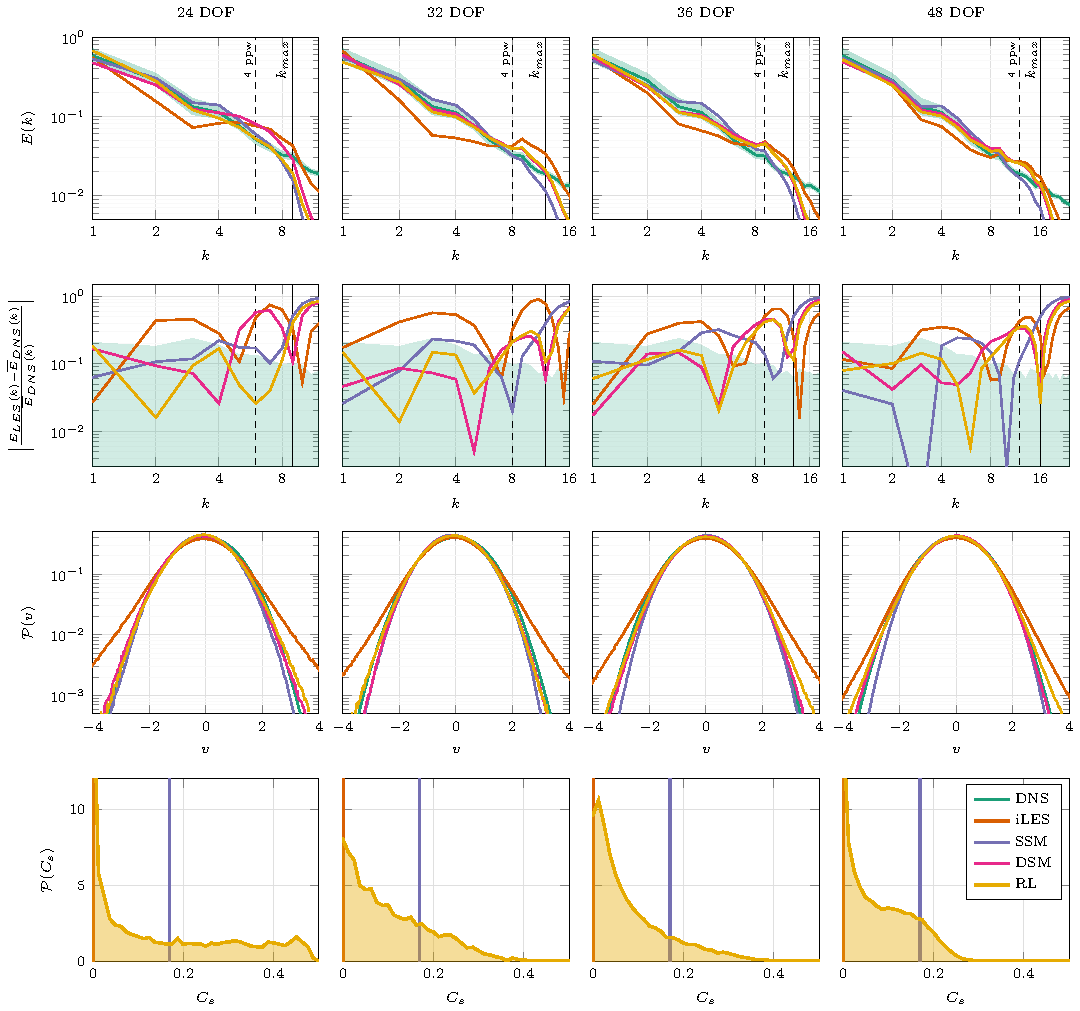
\includegraphics[width=\textwidth]{tikz_double_column/draft-figure6.pdf}
  \caption{Results for the RL models trained on $Re_{\lambda}\approx180$ evaluated on a HIT flow with $Re_{\lambda}\approx240$. Reported are (from top to bottom) the averaged energy spectra over the wavenumbers $k$, the relative error of the energy spectra with respect to the DNS solution, the distributions $\mathcal{P}(\cdot)$ of the velocity fluctuations, and the distribution of the predicted $C_s$ parameters. The results for the underlying DNS solution as well as an implicitly modeled LES (iLES), the SSM with $C_s=0.17$ and the DSM are shown for comparison. The shaded area for the DNS energy spectrum indicates the maximum and minimum amplitudes observed for each mode. The wavenumber that is resolved by the discretization with 4 points per wavelength is shown dashed and the maximum wavenumber used for optimization $k_{max}$ is indicated with a solid black line.}
  \label{fig:generalization_re}
\end{figure*}

The results in \figref{fig:generalization_re} indicate that the trained models can indeed generalize to flows at higher Reynolds numbers.
Most importantly, the RL models still provide long-term stable simulations.
The RL models show similar behavior as for the Reynolds number seen during training. 
For the 32 DOF, 36 DOF and 48 DOF cases the RL models is able to reproduce the energy spectrum more accurately than the implicit model and the SSM, but with similar accuracy as the DSM. 
Interestingly, the DSM and RL models exhibit a similar buildup of energy near the cutoff wavenumber, which might indicate that these models lack sufficient dissipation.
Moreover, the RL model sill outperforms the other models and especially the DSM for the 24 DOF simulation, where the modeling assumptions of the SSM and DSM most probably do not hold.

These results are very promising, since they indicate that the trained RL policies are able to extrapolate to other Reynolds numbers (at least to a moderate extent).
The trained policies are thus able to generalize to higher Reynolds number flows as well as other LES resolutions, while matching or even improving on the performance of the DSM, which is known to provide outstanding results for HIT flows.
